\documentclass{article}
\usepackage[ backend=biber]{biblatex}
\addbibresource{prop.bib}
\ExecuteBibliographyOptions{sorting=none,maxbibnames=5,doi=false,isbn=false,url=false}
\usepackage{fullpage}
\usepackage[utf8]{inputenc}
\usepackage{tensor}
\usepackage{url}
\usepackage{amsmath}
\usepackage{amssymb}
\usepackage{amsthm}
\usepackage{mathrsfs}
\usepackage{bbm}
\usepackage{bbold}
\usepackage{wesa}
\usepackage{graphicx}

\theoremstyle{remark}
\newtheorem{example}{Example}
\newtheorem{definition}{Definition}
\newtheorem{cor}{Corollary}
\newtheorem{lemma}{Lemma}
\newtheorem{thm}{Theorem}
\newtheorem{case}{Case}
\newtheorem{conjecture}{Conjecture}
\newtheorem{problem}{Problem}
\newtheorem{claim}{Claim}

\newcommand{\Hilb}{\mathcal{H}}
\newcommand{\events}{\ensuremath{\mathcal{E}}}
\newcommand{\qevents}{\ensuremath{\mathcal{E}}}
\newcommand{\pmeas}{\ensuremath{\mu}}
\newcommand{\imposs}{{\mbox{\wesa{impossible}}}}
\newcommand{\likely}{{\mbox{\wesa{likely}}}}
\newcommand{\unlikely}{{\mbox{\wesa{unlikely}}}}
\newcommand{\necess}{{\mbox{\wesa{certain}}}}
\newcommand{\overflow}{{\mbox{\wesa{overflow}}}}
\newcommand{\unknown}{{\mbox{\wesa{unknown}}}}
\newcommand{\bra}[1]{{\left\langle{#1}\right\vert}}
\newcommand{\ket}[1]{{\left\vert{#1}\right\rangle}}
\newcommand{\op}[2]{\ensuremath{\left\vert{#1}\middle\rangle\middle\langle{#2}\right\vert}}
\newcommand{\proj}[1]{\op{#1}{#1}}
\def\C{{\mathbb{C}}}
\newcommand{\ps}{\texttt{+}}
\newcommand{\ms}{\texttt{-}}
\newcommand{\ip}[2]{\ensuremath{\left\langle{#1}\middle\vert{#2}\right\rangle}}
\newcommand{\Tr}{\mathop{\mathrm{Tr}}\nolimits}
\newcommand{\rme}{\mathrm{e}}
\newcommand{\rmi}{\mathrm{i}}

%% \title{Computational Quantum Probabilities}
%% \title{Measurement and Probability in Fuzzy Quantum Theories}
\title{Measurement and Probability in Fuzzy Quantum Theories}
\date{}
\begin{document}
\maketitle 

%%%%%%%%%%%%%%%%%%%%%%%%%%%%%%%%%%%%%%%%%%%%%%%%%%%%%%%%%%%%%%%%%%%%%%%%%%%%%%
\section{Overview, Objectives, and Expected Significance} 

This is a \emph{theoretical} investigation of \emph{experimental}
physics using \emph{computational} methods. All experiments and
computations are processes bounded in space, time, energy, and other
resources. Yet, for centuries, the mathematical formalization of such
processes has been founded on the infinitely precise real or complex
numbers. Indeed, almost every description of quantum mechanics,
quantum computation, or quantum experiments refers to entities such as
$e$, $\pi$, $\sqrt{2}$, etc. From a computational perspective, such
numbers do not exist in their entirety ``for free.''  For example, the
state of the art algorithms for computing the $n$th binary digit of~$\pi$
require on the order of $O(n\log^{O(1)}(n))$
operations~\cite{journals/moc/BaileyBP97}. In other words, simply
referring to the $n$th digit of $\pi$ requires more and more resources
as $n$ gets larger. Taking such resource bounds in consideration is
what founded computer science as a discipline and is crucial for
understanding the very nature of computation and, following
Feynman~\cite{Feynman1982Simulating}, Landauer~\cite{Landauer1996188},
and others, for understanding the very nature of physical processes.

We propose to revisit quantum mechanics, quantum information, and
quantum computation from this resource-aware perspective. Our initial
result in that domain showed how subtle the issues can be~\cite{usat}:
a straightforward replacement of the complex numbers by a finite field
yields a variant of quantum mechanics in which computationally hard
problems like UNIQUE-SAT (which decides whether a given Boolean
formula is unsatisfiable or has exactly one satisfying assignment) can
be deterministically solved in constant time. To eliminate such
unrealistic theories requires delicate analysis of the structure of
the Hilbert space, the process of observation, and the notion of
probability teasing apart their reliance on the infinitely precise
real numbers~\cite{geometry2013,DQT2014}. In this proposal, our aim is
to shift focus from the infinitely-specified but not directly
observable quantum states, to observable measurable properties of
quantum systems and their probabilities. Furthermore, we insist that
our theories of measurement and probability only refer to finitely
communicable evidence within feasible computational bounds. It follows
that states, observations, and probabilities all become ``fuzzy'',
i.e., specified by intervals of confidence that can only increase in
precision if the available resources increase proportionally. Our
notion of ``fuzzy quantum mechanics'' is related to existing
work~\cite{GranikCaulfield1996,Pykacz2013,SNL2009,Gudder2005,aerts1993physical}
but, as will be explained in more detail, is distinguished by its
computational character.

We will begin by reviewing existing work that recasts classical
probability spaces in a resource-aware setting and move to our
proposal which, briefly speaking, aims at recasting quantum
probability and hence quantum measurement to a corresponding
resource-aware setting. In particular, we plan on addressing the
Meyer-Mermin debate~\cite{PhysRevLett.83.3751, Mermin1999,
  BarrettKent2004} on the impact of finite precision measurements on
the relevance of the Kochen-Specker
theorem~\cite{kochenspecker1967,Redhead1987-REDINA,peres1995quantum,Jaeger2007}.
We argue that no matter
what the results are their impact will be strong. Positive results
that formulate a computable, with clear resource bounds, theory of
quantum measurement and quantum probability would be essential for
understanding and realizing quantum computation. Any negative results
would redirect research that aims at realizing quantum computation to
other approaches. At an intellectual level, the results will solve or
clarify several paradoxes in quantum mechanics, quantum information,
computability, and complexity theory.

%%%%%%%%%%%%%%%%%%%%%%%%%%%%%%%%%%%%%%%%%%%%%%%%%%%%%%%%%%%%%%%%%%%%%%%%%%%%%%
\section{Background I: Classical Probability}

A \emph{probability space} specifies the necessary conditions for
reasoning coherently about collections of uncertain
events~\cite{Kolmogorov1950,Shafer1976,Griffiths2003,Swart2013}.  We
review the conventional presentation of probability spaces and then
discuss the computational resources needed to estimate probabilities.

%%%
\subsection{Classical Probability Spaces}

The conventional definition of a probability space builds upon the
field of real numbers. In more detail, a probability space consists of
a \emph{sample space} $\Omega$, a space of \emph{events}~$\events$,
and a \emph{probability measure}~$\pmeas$ mapping events in $\events$
to the real interval $[0,1]$. We will only consider \emph{finite} sets
of events and restrict our attention to non-empty finite sets $\Omega$
as the sample space. The space of events $\events$ includes every
possible subset of $\Omega$: it is the
powerset~$2^{\Omega}=\left\{ E ~\middle|~ E\subseteq\Omega\right\}
$.
For future reference, we emphasize that events are the primary notion
of interest and that the sample space is a convenient artifact that
allows us to treat events as sets obeying the laws of Boolean
algebra~\cite{Boole1948,Redhead1987-REDINA,Griffiths2003}.

\begin{definition}[Probability Measure]\label{def:ClassicalProbabilitySpace}
  Given the set of events $\events$, a \emph{probability measure} is a
  function $\pmeas:\events\rightarrow[0,1]$ such that:
\begin{itemize}
\item $\pmeas(\emptyset)=0$,
\item $\pmeas(\Omega)=1$, 
\item for every event $E$,
  $\pmeas\left(\Omega\backslash E\right)=1-\pmeas\left(E\right)$ where
  $\Omega\backslash E$ is the complement event of $E$, and
\item for every collection $\left\{ E_{i}\right\} _{i=1}^{N}$ of
  pairwise disjoint events,
  $\pmeas\left(\bigcup_{i=1}^{N}E_{i}\right)=\sum_{i=1}^{N}\pmeas(E_{i})$.
\end{itemize}
\end{definition}
\noindent There is some redundancy in the definition that will be useful when
moving to quantum probability spaces. 

\begin{example}[Two-coins experiment]\label{ex1} Consider an
  experiment that tosses two coins. We have four possible outcomes
  that constitute the sample space $\Omega=\{HH,HT,TH,TT\}$. There are
  16 total events including the event $\{HH,HT\}$ that the first coin
  lands heads up, the event $\{HT,TH\}$ that the two coins land on
  opposite sides, and the event $\{HT,TH,TT\}$ that at least one coin
  lands tails up. Here is a possible probability measure for these
  events:
\[
\begin{array}{c@{\qquad\qquad}c}
\begin{array}{rcl}
\pmeas(\emptyset) & = & 0\\
\pmeas(\{HH\}) & = & 1/3\\
\pmeas(\{HT\}) & = & 0\\
\pmeas(\{TH\}) & = & 2/3\\
\pmeas(\{TT\}) & = & 0\\
\pmeas(\{HH,HT\}) & = & 1/3\\
\pmeas(\{HH,TH\}) & = & 1\\
\pmeas(\{HH,TT\}) & = & 1/3
\end{array} & \begin{array}{rcl}
\pmeas(\{HT,TH\}) & = & 2/3\\
\pmeas(\{HT,TT\}) & = & 0\\
\pmeas(\{TH,TT\}) & = & 2/3\\
\pmeas(\{HH,HT,TH\}) & = & 1\\
\pmeas(\{HH,HT,TT\}) & = & 1/3\\
\pmeas(\{HH,TH,TT\}) & = & 1\\
\pmeas(\{HT,TH,TT\}) & = & 2/3\\
\pmeas(\{HH,HT,TH,TT\}) & = & 1
\end{array}\end{array}
\]
\end{example}

\noindent It is useful to think that this probability measure is
completely determined by the ``reality'' of the two coins in question
and their characteristics, in the sense that each pair of coins
induces a measure, and each measure must correspond to some pair of
coins. The measure above would be induced by two particular coins such
that the first coin is twice as likely to land tails up than heads up
and the second coin is double-headed. In a strict computational
or experimental setting, one should question the reliance of the
definition of probability space on the uncountable and
uncomputable~\cite{Turing01011937,Ziegler2007,weihrauch2012computable}
real interval $[0,1]$. This interval includes numbers like
$0.h_{1}h_{2}h_{3}\ldots$ where $h_{i}$ is 1 or 0 depending on whether
Turing machine $M_{i}$ halts or not. Such numbers cannot be
computed. This interval also includes numbers like $\frac{\pi}{4}$
which can only be computed with increasingly large resources as the
precision increases. Therefore, in a resource-aware computational or
experimental setting, it is more appropriate to consider probability
measures that map events to a set of elements computable with a fixed
set of resources. We expand on this observation in the next section
and then recall its formalization using interval-valued probability
measures~\cite{Weichselberger2000,JamisonLodwick2004}.

%%%%%
\subsection{Measuring Probabilities: Buffon's Needle Problem\label{subsec:Measuring-Probabilities:-Buffon}}

In the previous example, we assumed the probability~$\pmeas(E)$ of
each event~$E$ is known a priori. In reality, although each event is
assumed to have a probability, the exact value of $\pmeas(E)$ may not
be known. According to the \emph{frequency interpretation of
  probability} (which we will revisit when moving to the quantum
case), to determine the probability of an event, we run $N$
independent trials which gives us an approximation of the (assumed)
``true'' or ``real'' probability. Let $x_{i}$ be 1 or 0 depending on
whether the event~$E$ occurs in the $i$-th trial or not, then
$\pmeas(E)$ could be approximated to given accuracy~$\epsilon>0$ by
the relative frequency~$\frac{1}{N}\sum_{i=1}^{N}x_{i}$ with the
probability converging to one as $N$ goes to infinity, i.e.,
\[
\forall\epsilon>0,\lim_{N\rightarrow\infty}\pmeas\left(\left|\pmeas(E)-\frac{1}{N}\sideset{}{_{i=1}^{N}}\sum x_{i}\right|<\epsilon\right)=1\textrm{ .}
\]
This fact is called the law of large numbers~\cite{Bernoulli2006,Kolmogorov1950,Uspensky1937,Shafer1976,544199}.

Let's look at a concrete example. Suppose we drop a needle of length
$\ell$ onto a floor made of equally spaced parallel lines a distance
$h$ apart, where $\ell<h$. It is a known fact that the probability of
the needle crossing a line is
$\frac{2\ell}{\pi
  h}$~\cite{Buffon1777,DeMorgan1872,Hall1873,Uspensky1937}.
Consider an experimental setup consisting of a collection of $N$
identical needles of length $\ell$. We throw the $N$ needles one
needle at a time, and observe the number $M$ of needles that cross a
line, thus estimating the probability of a needle crossing a line to
be $\frac{M}{N}$. In an actual experiment with $500$ needles and the
ratio $\frac{\ell}{h}=0.75$~\cite{Hall1873}, it was found that $236$
crossed a line so the relative frequency is $0.472$ whereas the
idealized mathematical probability is $0.4774\ldots$.  In a larger
experiment with $5000$ needles and the ratio
$\frac{\ell}{h}=0.8$~\cite{Uspensky1937}, the relative frequency was
calculated to be $0.5064$ whereas the idealized mathematical
probability is $0.5092\ldots$. We see that the observed probability
approaches $\frac{2\ell}{\pi h}$ but only if \emph{larger and larger
  resources} are expended. These resource considerations suggest that
it is possible to replace the real interval $[0,1]$ with rational
numbers up to a certain precision related to the particular experiment
in question. There is clearly a connection between the number of
needles and the achievable precision: in the hypothetical experiment
with 3 needles, it is not sensible to retain 100 digits in the
expansion of $\frac{2\ell}{\pi h}$.

There is another more subtle assumption of unbounded computational
power in the experiment. We are assuming that we can always determine
with certainty whether a needle is crossing a line. But ``lines'' on
the the floor have thickness, their distance apart is not exactly $h$,
and the needles' lengths are not all absolutely equal to $\ell$.
These perturbations make the events ``fuzzy.'' Thus, in an experiment
with limited resources, it is not possible to talk about the idealized
event that exactly $M$ needles cross lines as this would require the
most expensive needles built to the most precise accuracy, laser
precision for drawing lines on the floor, and the most powerful
microscopes to determine if a needle does cross a line. Instead we
might talk about the event that $M-\delta$ needles evidently cross
lines and $M+\delta'$ needles plausibly cross lines where $\delta$ and
$\delta'$ are resource-dependent approximations. This fuzzy notion of
events leads to probabilities being only calculable within intervals
of confidence reflecting the certainty of events and their
plausibility. This is indeed consistent with published experiments: in
an experiment with $3204$ needles and the ratio
$\frac{\ell}{h}=0.6$~\cite{DeMorgan1872}, $1213$ needles clearly
crossed a line and $11$ needles were close enough to plausibly be
considered as crossing the line: we would express the probability in
this case as the interval
$\left[\frac{1213}{3204},\frac{1224}{3204}\right]$ expressing that we
are certain that the event has probability at least
$\frac{1213}{3204}$ but it is possible that it would have probability
$\frac{1224}{3204}$.

%%%%%
\subsection{Classical Interval-Valued Probability Measures}

As motivated above, an event $E_{1}$ may have an interval of
probability $[l_{1},r_{1}]$. Assume that another disjoint event
$E_{2}$ has an interval of probability $[l_{2},r_{2}]$, what is the
interval of probability for the event $E_{1}\cup E_{2}$? The answer is
somewhat subtle: although it is possible to use the sum of the
intervals $[l_{1}+l_{2},r_{1}+r_{2}]$ as the combined probability, one
can find a much tighter interval if information \emph{against} the
event (i.e., information about the complement event) is also taken
into consideration. Formally, for a general event $E$ with probability
$[l,r]$, the evidence that contradicts $E$ is evidence supporting the
complement of $E$.  The complement of $E$ must therefore have
probability $\left[1-r,1-l\right]$ which we abbreviate
$\left[1,1\right]-\left[l,r\right]$.  Given a sample space~$\Omega$
and its set of events~$\events$, a
function~$\bar{\mu}:\events\rightarrow[0,1]$ is a classical
interval-valued probability measure if and only if $\bar{\mu}$
satisfies the following conditions~\cite{JamisonLodwick2004} where the
last line uses $\subseteq$ to allow for tighter intervals that exploit
the complement event:
\begin{itemize}
\item $\bar{\mu}(\emptyset)=[0,0]$.
\item $\bar{\mu}(\Omega)=[1,1]$. 
\item For any event $E$,
  $\bar{\mu}\left(\Omega\backslash E\right)=\left[1,1\right]-\bar{\mu}\left(E\right)$
\item For a collection $\left\{ E_{i}\right\} _{i=0}^{N}$ of pairwise
  disjoint events, we have
  $\bar{\mu}\left(\bigcup_{i=0}^{N}E_{i}\right)\subseteq\sum_{i=0}^{N}\bar{\mu}\left(E_{i}\right)$.
\end{itemize}

\begin{example}[Two-coin experiment with interval probability]
\label{ex3} We split the unit interval $[0,1]$ in the following
four closed sub-intervals: $[0,0]$ which we call \imposs, $[0,\frac{1}{2}]$
which we call \unlikely, $[\frac{1}{2},1]$ which we call \likely,
and $[1,1]$ which we call \necess. Using these new values, we can
modify the probability measure of Ex.~\ref{ex1} by mapping each
numeric value to the smallest sub-interval containing it to get the
following: 
\[
\begin{array}{c@{\qquad\qquad}c}
\begin{array}{rcl}
\bar{\mu}(\emptyset) & = & \imposs\\
\bar{\mu}(\{HH\}) & = & \unlikely\\
\bar{\mu}(\{HT\}) & = & \imposs\\
\bar{\mu}(\{TH\}) & = & \likely\\
\bar{\mu}(\{TT\}) & = & \imposs\\
\bar{\mu}(\{HH,HT\}) & = & \unlikely\\
\bar{\mu}(\{HH,TH\}) & = & \necess\\
\bar{\mu}(\{HH,TT\}) & = & \unlikely
\end{array} & \begin{array}{rcl}
\bar{\mu}(\{HT,TH\}) & = & \likely\\
\bar{\mu}(\{HT,TT\}) & = & \imposs\\
\bar{\mu}(\{TH,TT\}) & = & \likely\\
\bar{\mu}(\{HH,HT,TH\}) & = & \necess\\
\bar{\mu}(\{HH,HT,TT\}) & = & \unlikely\\
\bar{\mu}(\{HH,TH,TT\}) & = & \necess\\
\bar{\mu}(\{HT,TH,TT\}) & = & \likely\\
\bar{\mu}(\{HH,HT,TH,TT\}) & = & \necess
\end{array}\end{array}
\]
Despite the absence of infinitely precise numeric information, the
probability measure is quite informative: it reveals that the second
coin is double-headed and that the first coin is biased. To understand
the $\subseteq$-condition, consider the following calculation:
\begin{eqnarray*}
\bar{\mu}(\{HH\})+\bar{\mu}(\{HT\})+\bar{\mu}(\{TH\})+\bar{\mu}(\{TT\})
&=& \imposs+\unlikely+\imposs+\likely\\
&=& \left[0,0\right]+\left[0,\frac{1}{2}\right]+\left[0,0\right]+\left[\frac{1}{2},1\right]\\
&=& \left[\frac{1}{2},\frac{3}{2}\right]
\end{eqnarray*}
If we were to equate $\bar{\mu}(\Omega)$ with the sum of the individual
probabilities, we would get that $\bar{\mu}(\Omega)=\left[\frac{1}{2},\frac{3}{2}\right]$.
However, using the fact that $\bar{\mu}(\emptyset)=\imposs$, we have
$\bar{\mu}\left(\Omega\right)=1-\bar{\mu}\left(\emptyset\right)=\necess=[1,1]$.
This interval is tighter and a better estimate for the probability
of the event $\Omega$, and of course it is contained in $[\frac{1}{2},\frac{3}{2}]$.
However it is only possible to exploit the information about the complement
when all four events are combined. Thus the $\subseteq$-condition
allows us to get an estimate for the combined event from each of its
constituents and then gather more evidence knowing the aggregate
event.
\end{example}

%%%%%%%%%%%%%%%%%%%%%%%%%%%%%%%%%%%%%%%%%%%%%%%%%%%%%%%%%%%%%%%%%%%%%%%%%%%%%%
\section{Background II: Quantum Probability}
 
The mathematical framework of classical probability above assumes that
there exists a predetermined set of events that are independent of the
particular experiment --- classical physics is
non-contextual. However, even in classical situations, the structure
of the event space is often only partially known and the precise
dependence of two events on each other cannot, a priori, be determined
with certainty. In the quantum framework, this partial knowledge is
compounded by the fact that there exist non-commuting events which
cannot happen simultaneously. To accommodate these more complex
situations, conventional approaches to quantum probability abandon the
sample space~$\Omega$ and reason directly about events which are
generalized from plain sets to projection operators. A quantum
probability space therefore consists of just two components: a set of
events $\qevents$ often formalized as projection operators and a
probability measure $\mu:\qevents\rightarrow[0,1]$ formalized using
the Born rule.

%%%%%
\subsection{Quantum Events}

\begin{definition}[Projection Operators; Orthogonality~\cite{10.2307/2308516,Redhead1987-REDINA,peres1995quantum,Griffiths2003,Swart2013}]
  \label{def:Projection} Given a Hilbert space $\Hilb$, an event (an
  experimental proposition~\cite{BirkhoffVonNeumann1936}, a
  question~\cite{10.2307/2308516,DBLP:journals/corr/abs-0910-2393}, or
  an elementary quantum test~\cite{peres1995quantum}) is represented
  as a (self-adjoint or orthogonal~\cite {Griffiths2003,Maassen2010})
  projection operator $P:\Hilb\rightarrow\Hilb$ onto a linear subspace
  of $\Hilb$. The following define projections and list some of their properties:
\begin{itemize}
\item $\mathbb{0}$ is a projection. 
\item For any pure state~$\ket{\psi}$, $\proj{\psi}$ is a projection
operator. 
\item Projection operators $P_{0}$ and $P_{1}$ are \emph{orthogonal}
  if $P_{0}P_{1}=P_{1}P_{0}=\mathbb{0}$. The sum of two projection
  operators~$P_{0}+P_{1}$ is also a projection operator if and only if
  they are orthogonal.
\item Conversely, every projection~$P$ can be expressed as
  $\sum_{j=1}^{N}\proj{\psi_{j}}$, where $P$ actually projects onto
  the linear subspace with orthonormal
  basis~$\left\{ \ket{\psi_{j}}\right\} _{j=1}^{N}$.
\item A set of projections $\left\{ P_{i}\right\} _{i=1}^{N}$ is
  called an \emph{ideal measurement} if it is a partition of the
  identity, i.e., $\sum_{i=1}^{N}P_{i}=\mathbb{1}$~\cite{Swart2013}.
  In this case, projections $\left\{ P_{i}\right\} _{i=1}^{N}$ must
  be mutually orthogonal~\cite{Griffiths2003} and $N$ must correspond
  to the dimension of the Hilbert space.
\item If $P$ is a projection operator, then $\mathbb{1}-P$ is also a
  projection operator, called its \emph{complement}. It is orthogonal to
  $P$, and corresponds to the complement event~$\Omega\backslash E$ in
  classical probability~\cite{Griffiths2003}.
\item Projection operators $P_{0}$ and $P_{1}$ \emph{commute} if $P_{0}P_{1}=P_{1}P_{0}$.
The product of two projection operators~$P_{0}P_{1}$ is also a projection
operator if and only if they commute. This corresponds to the classical
intersection between events~\cite{peres1995quantum,Griffiths2003}. 
\item For two commuting projection operators $P_{0}$ and $P_{1}$,
  their \emph{disjunction}~$P_{0}\vee P_{1}$ is defined to be
  $P_{0}+P_{1}-P_{0}P_{1}$~\cite{Griffiths2003}.
\end{itemize}
\end{definition}

\begin{example}[One-qubit quantum probability space] Consider a
  one-qubit Hilbert space with each event interpreted as a possible
  post-measurement state. For example, the event $\proj{0}$ indicates
  that the post-measurement state will be $\ket{0}$; the probability
  of such an event depends on the current state; the event $\proj{1}$
  indicates that the post-measurement state will be $\ket{1}$; the
  event $\proj{\ps}$ where
  $\ket{\ps}=\frac{1}{\sqrt{2}}(\ket{0}+\ket{1})$ indicates that the
  post-measurement state will be $\ket{\ps}$; the event
  $\mathbb{1}=\proj{0}+\proj{1}$ indicates that the post-measurement
  state will be a linear combination of $\ket{0}$ and $\ket{1}$ and is
  clearly certain; finally the empty event $\mathbb{0}$ states that
  the post-measurement state will be the empty state and is
  impossible. As in the classical case, a probability measure is a
  function that maps events to $[0,1]$. Here is a partial
  specification of a possible probability measure that would be
  induced by a system whose current state is $\ket{0}$:
\[
\mu\left(\mathbb{0}\right)=0,\quad
\mu\left(\mathbb{1}\right)=1,\quad
\mu\left(\proj{0}\right)=1,\quad
\mu\left(\proj{1}\right)=0,\quad
\mu\left(\proj{\ps}\right)=1/2,\quad
\ldots
\]
Note that, similarly to the classical case, the probability of
$\mathbb{1}$ is 1 and the probability of collections of orthogonal
events (e.g., $\proj{0}+\proj{1}$) is the sum of the individual
probabilities.  A collection of non-orthogonal events (e.g.,
$\proj{0}$ and $\proj{\ps}$) is however not even a valid event. In the
classical example, we argued that each probability measure is uniquely
determined by two actual coins. A similar (but much more subtle)
argument is valid also in the quantum case. By postulates of quantum
mechanics and Gleason's theorem, it turns out that for large enough
quantum systems, each probability measure is uniquely determined by an
actual quantum state as discussed next.
\end{example}

%%%%%
\subsection{Quantum Probability Measures}

Given our setup, the definition of a quantum probability measure is a
small variation on the classical definition. 

\begin{definition}[Quantum Probability Measure~\cite{10.2307/2308516,gleason1957,Redhead1987-REDINA,Maassen2010}]\label{def:QuantumProbabilitySpace}
Given a Hilbert space $\Hilb$ with its set of events~$\events$,
a \emph{quantum probability measure} is a function~$\mu:\events\rightarrow[0,1]$
such that: 
\begin{itemize}
\item $\mu(\mathbb{0})=0$. 
\item $\mu(\mathbb{1})=1$. 
\item For any projection $P$, $\mu\left(\mathbb{1}-P\right)=1-\mu\left(P\right)$.
\item For a set of mutually orthogonal projections $\left\{ P_{i}\right\} _{i=1}^{N}$,
we have $\mu\left(\sum_{i=1}^{N}P_{i}\right)=\sum_{i=1}^{N}\mu\left(P_{i}\right)$.
\end{itemize}
\end{definition}

\noindent A quantum probability measure can be easily constructed if
one knows the current state of the quantum system by using the Born
rule~\cite{Born1983,Mermin2007,Jaeger2007}.  Specifically, for each
pure normalized quantum state $\ket{\phi}$, the Born rule induces a
probability measure $\mu_{\phi}^{B}$ defined as
$\mu_{\phi}^{B}(P)=\ip{\phi}{P\phi}$. The situation generalizes to
mixed states $\rho = \sum_{j=1}^{N}q_{j}\proj{\phi_{j}}$, where
$\sum_{j=1}^{N}q_{j}=1$ in which case the generalized Born rule
induces a probability measure $\mu_{\rho}^{B}$ defined
as follows~\cite{peres1995quantum,544199,Jaeger2007}:
\[
\mu_{\rho}^{B}\left(P\right) = 
\Tr\left(\rho P\right) = 
\sideset{}{_{j=1}^{N}}\sum q_{j}\mu_{\phi_{j}}^{B}\left(P\right)
\]
Conversely every probability measure must be of this form.

\begin{thm}[Gleason's
  theorem~\cite{gleason1957,Redhead1987-REDINA,peres1995quantum}]\label{cor:Gleason's}In
a Hilbert space $\Hilb$ of dimension $d\geq3$, given a quantum probability
measure~$\mu:\events\rightarrow[0,1]$, there exists a unique mixed
state~$\rho$ such that $\mu=\mu_{\rho}^{B}$.
\end{thm}

%%%%%
\subsection{Measuring Quantum Probabilities}

By using the law of large numbers, quantum probabilities can be also
estimated by relative frequencies. For example, if we want to know the
probability of ``spin up'' in a Stern-Gerlach
experiment~\cite{Stern1988,peres1995quantum,544199,Griffiths2003}, we
can put a beam of silver atoms in a highly inhomogeneous magnetic
field, and count the number of atoms deflects up. Ideally, if the
local field of strength directs to the $z$-axis, and all particles
have the same velocity, the Stern-Gerlach experiment only produces two
spots corresponding to $\ket{0}$ and $\ket{1}$. Notice that whenever
the magnetic field of the Stern-Gerlach is fixed, i.e., an ideal
measurement is picked, measuring the spin is exactly the same as
tossing a coin. In other words, if someone claims to be tossing a coin
behind a veil, and only shows the resulting heads or tails, we cannot
distinguish whether the results are really deriving from tossing a
coin, or by running a Stern-Gerlach experiment, and showing the head,
the tail, or the side of coin if the silver atoms is spin up, spin
down, or just hit the middle, respectively. Following our theme, a
Stern-Gerlach experiment requires significant resources to keep the
local field of strength directing to the $z$-axis precisely, to keep
the atoms having almost the same velocity, and to point out the exact
position each particle landed on. If the field of strength does not
perfectly direct to the $z$-axis, we do not really test the quantum
event we want to test. Even if the field of strength perfectly directs
to the $z$-axis, the variant velocity makes spots broader and more
washed out. Together with the precision limit of the detector, it may
sometimes be hard to decide a particle corresponding to which state.

%%%%%%%%%%%%%%%%%%%%%%%%%%%%%%%%%%%%%%%%%%%%%%%%%%%%%%%%%%%%%%%%%%%%%%%%%%%%%%
\section{Proposal: General Plan} 

A major aim of this proposal is to recast quantum probability and
measurement in a computational resource-aware setting. Our vision is
to unify the strands above in a novel way as explained in this
section. We start with some immediate observations that justify the
rest of the development. 

\begin{itemize}

\item If we insist that probabilities cannot be infinitely precise and
  are bound to be approximations represented by intervals of
  confidence, then by Gleason's theorem, quantum states themselves
  cannot be infinitely precise. This raises an important philosophical
  question with immense practical relevance in the context of quantum
  computing. The question, which we could largely bypass in the
  classical case, is whether there is, in the background of all the
  measurements and probabilities, a ``real'' infinitely-precise
  quantum state that is being approximated and that, in principle, can
  be more and more accurately described given more and more
  resources. In other words, does a Gleason, Bell, or Kochen-Specker
  theorem still hold in a world with finite resources?  The answer
  will have to be \emph{no} if we are to respect these major theorems
  of quantum mechanics and quantum information. Thus our first radical
  departure from the conventional case will be that the quantum state
  itself must be fuzzy in some sense to be formalized.

\item Going further we actually have to concede not just the infinite
  accuracy of the quantum state, but its very existence as a ``real''
  entity that exists independently of measurements and
  probabilities. The reasons for this second radical position are as
  follows. First arguments embedded in the proof of the Kochen-Specker
  theorem essentially rule out the existence of a sample space as the
  probabilities of events cannot be consistently expressed using core
  assignments to elements of the sample space. Second, the frequency
  interpretation of probability which is already problematic in the
  classical case, becomes untenable in the quantum case. In both
  cases, but much more in the quantum case, it is much more sensible
  to interpret probability in the Bayesian sense as ``lack of
  knowledge''. This, and similar arguments elegantly expressed by
  recent work on Quantum Bayesianism~\cite{Fuchs2010,VonBaeyer2016},
  suggest that the quantum state is more like an interactive system in
  computer science parlance. In other words, the state is only
  determined by its interactions with the environment or observers. A
  rough but useful analogy in the context of computer science would be
  a web server: the state of such a system cannot be said to exist
  independently of the interactions with clients; each interaction
  with a client determines a future state of the system and may affect
  future interactions. Crucially, each client may have a
  \emph{different} view of the web server that is consistent with
  their own history of interactions. This computational perspective
  agrees with the philosophical position of QBism~\cite{VonBaeyer2016}
  that asserts that the quantum state is subjective: each observer has
  a different view of the quantum system that is consistent with their
  previous observations and that allows that observer, independently
  of other observers, to assign beliefs (i.e., probabilities) to
  possible future interactions.

\end{itemize} 

%%%%
\subsection{Proposed Activity I: Quantum States as Interactive Processes} 

The early formalization of the process of computing using Turing
machines~\cite{Turing01011937} or the
$\lambda$-calculus~\cite{Barendregt:Lambda} viewed a computation as
realizing a mathematical function. From our perspective, the most
important consequence of this view is that the properties of the
computed function existed independently of any observation,
calculation, or interaction. For example, a function is
\emph{injective} or not independently of any observation. An agent can
only interact with the computation by asking questions regarding its
input-output behavior and although such interaction would reveal
fragments of the computed function and its innate properties it could
not change it or affect it in any way.

In a series of breakthrough papers that led to his Turing
Award~\cite{Milner:1993:EIT:151233.151240}, Milner argued that this
``closed system'' view of computation is too limiting as it cannot
adequately describe the increasingly pervasive \emph{interactive
  computations}. Milner explained that ``concurrency requires a new
conceptual framework'' and ``not merely an extension of the repertoire
of entities and constructions which explain sequential computing.'' In
his Turing Award lecture, he gives the following simple but compelling
example. Consider the following two programs:
\begin{verbatim}
Program P1: x := 1; x := x + 1 
Program P2: x := 2
\end{verbatim}
As closed systems, these two programs define the same relation, namely
the one that maps an input memory to an updated memory in which the
location named \verb|x| is assigned the value \verb|2|. An observer
with the ability of inquire about the value of \verb|x| at the end of
the computation cannot distinguish the two programs. But place the
programs in an environment which may involve interactions and the
equivalence is lost. Phrased in physical terms, we give the observer the
additional ability to access the location \verb|x| \emph{during} the
computation, not just to observe its final value. In computing terms,
we place each of the two programs \verb|P1| and \verb|P2| concurrently
with the program:
\begin{verbatim}
Program Q: x := 3
\end{verbatim}
In the combined system of \verb|P1| and \verb|Q| running concurrently,
the location \verb|x| may end up containing \verb|2|, \verb|3|, or
\verb|4|. But in the combined system of \verb|P2| and \verb|Q| running
concurrently, the location~\verb|x| can only end up containing
\verb|2| or \verb|3|. The lesson, phrased in physics terms, is that it
is not sensible to think of the properties of a system (like \verb|P1|
or \verb|P2|) independently of the observer (\verb|Q| in this
case). Indeed the observation \verb|x=4| cannot said to have an
existence independently from the interaction between \verb|P1| and
\verb|Q|: it really emerges or is created as part of the observation
process and is not a pre-existing ``element of reality''.

This phenomenon is hardly a surprise to computer scientists or
physicists but embracing it fully does have far-reaching
consequences. In computer science, the big shift was to abandon the
idea that a computation has inherent internal meaning, e.g.,
representing a pure mathematical function. Instead \emph{the meaning
  of a computational process is its observable behavior.} It is not
too difficult to imagine that, in the presence of multiple interacting
observers, the behavior observed by just one agent would appear to
involve hidden variables or action at a distance. The well-established
theory of observation of concurrent processes and their
equivalences~\cite{Hennessy1989} relies on neither.

\paragraph*{Research Question.} Is it possible to adapt the theory of
observation of concurrent processes to the study of quantum states and
confirm that the observations exhibit the same Bell-like correlations?

\paragraph*{Research Question.} The theory of observation of
concurrent processes and the theory of measurement in quantum
mechanics are superficially different. Is it possible to reformulate
them in a common language to benefit each theory from insights derived
from the other theory?

\paragraph*{Research Question.} Does the computational and hence
\emph{testable} hypothesis that the quantum state is nothing but an
interactive system agree with the QBism perspective providing a
resolution to the same paradoxes (e.g., EPR and Wigner's friend)?

%%%%%
\subsection{Proposed Activity II: Quantum Interval-valued Probability Measures}
 
This is the most developed part of our current investigation and is
more detailed.

Just as it is the case for Buffon's needles, estimating quantum
probabilities (e.g., in the case of a Stern-Gerlach experiment) with
increasing accuracy requires increasingly large resources.  Therefore,
given some finite resources, it is only possible to estimate the
quantum probabilities within an interval of confidence. It is
therefore natural to introduce the notion of an ``interval-valued
quantum probability measure'' that combines the definitions of
conventional quantum probability measures with classical
interval-probabilities.

\begin{definition}[Quantum Interval-valued Probability Measure]\label{def:QuantumInterval-valuedProbability}
  Given a Hilbert space $\Hilb$ with quantum events
  (projections)~$\events$, and a collection of
  intervals~$\mathscr{I}$, a \emph{quantum
    $\mathscr{I}$-interval-valued probability measure} is a
  function~$\bar{\mu}:\events\rightarrow\mathscr{I}$ such that:
\begin{itemize}
\item $\bar{\mu}(\mathbb{0})=\left[0,0\right]$. 
\item $\bar{\mu}(\mathbb{1})=\left[1,1\right]$. 
\item For any projection $P$, 
\begin{equation}
\bar{\mu}\left(\mathbb{1}-P\right)=\left[1,1\right]-\bar{\mu}\left(P\right)\textrm{ .}\label{eq:QuantumInterval-valuedProbability-Complement}
\end{equation}
\item For a set of mutually orthogonal projections $\left\{ P_{i}\right\} _{i=1}^{N}$,
we have:
\begin{equation}
\bar{\mu}\left(\sideset{}{_{i=1}^{N}}\sum P_{i}\right)\subseteq\sideset{}{_{i=1}^{N}}\sum\bar{\mu}\left(P_{i}\right)
\label{eq:QuantumInterval-valuedProbability-Inclusion}
\end{equation}
\end{itemize}
\end{definition}

It is easy to establish that quantum interval-valued probability
measures generalize conventional quantum probability measures. In
particular, any quantum probability measure can be recast as an
interval-valued measure using the three intervals $\left[0,0\right]$,
$\left[1,1\right]$ and \emph{$\left[0,1\right]$}, where
$\left[0,0\right]$ and $\left[1,1\right]$ are called \imposs~and
\necess~as before, and \emph{$\left[0,1\right]$} is called
\unknown~because it provides no information as follows. Given a
probability measure~$\mu:\events\rightarrow\left[0,1\right]$, we
define a quantum interval-valued probability
measure~$\bar{\mu}:\events\rightarrow\mathscr{I}$ by
$\bar{\mu}(P)=\iota\left(\mu(P)\right)$, where
$\iota:\left[0,1\right]\rightarrow\mathscr{I}$ is defined by
\[
\iota(x)=\begin{cases}
\necess & \textrm{if }x=1\textrm{ ;}\\
\imposs & \textrm{if }x=0\textrm{ ;}\\
\unknown & \textrm{otherwise.}
\end{cases}
\]

The interesting question is the converse one corresponding to
Gleason's theorem. Given an interval-valued probability measure, i.e.,
given observations done with finite resources, do these observations
uniquely determine a quantum state? Our initial investigations
indicate that the answer is \emph{no}.

\begin{definition}
  Given a quantum interval-valued probability
  measure~$\bar{\mu}:\events\rightarrow\mathscr{I}$:
\begin{itemize}
\item A \emph{core} of $\bar{\mu}$ is the set $\mathrm{core}\left(\bar{\mu}\right)=\left\{ \textrm{quantum probability measure }\pmeas:\events\rightarrow[0,1]\middle|\forall E\in\events.\pmeas\left(E\right)\in\bar{\mu}\left(E\right)\right\} $.
\item $\bar{\mu}$ is called convex if 
\begin{equation}
  \bar{\mu}\left(P_{0}\vee P_{1}\right)+\bar{\mu}\left(P_{0}P_{1}\right)\subseteq\bar{\mu}\left(P_{0}\right)+\bar{\mu}\left(P_{1}\right)\label{eq:QuantumInterval-valuedProbability-Convex}
\end{equation}
 for all commuting $P_{0},P_{1}\in\events$. 
\end{itemize}
\end{definition}

\begin{thm}\label{def:EmptyCoreQuantumInterval-valuedProbability}
There is a convex quantum interval-valued probability measure~$\bar{\mu}:\events\rightarrow\mathscr{I}$
such that $\mathrm{core}\left(\bar{\mu}\right)=\emptyset$.
\end{thm}

This theorem can be proved by the following example. 

\begin{example}[Three-dimensional quantum three-value interval-valued
probability measure]\label{ex:three-dimensional-three-value} Given
a three dimensional Hilbert space with an orthonormal basis $\left\{ \ket{0},\ket{1},\ket{2}\right\} $.
Consider\emph{ $\mathscr{I}=\left\{ \necess,\imposs,\unknown\right\} $}
and $\ket{\ps}=\frac{1}{\sqrt{2}}(\ket{0}+\ket{1})$, and $\ket{\ps'}=\frac{1}{\sqrt{2}}(\ket{0}+\ket{2})$.
Let 
\begin{eqnarray*}
\bar{\mu}(\mathbb{0})=\bar{\mu}(\proj{0})=\bar{\mu}(\proj{\ps})=\bar{\mu}(\proj{\ps'}) & = & \imposs\textrm{ ,}\\
\bar{\mu}(\mathbb{1})=\bar{\mu}(\mathbb{1}-\proj{0})=\bar{\mu}(\mathbb{1}-\proj{\ps})=\bar{\mu}(\mathbb{1}-\proj{\ps'}) & = & \necess\textrm{ ,}\\
\bar{\mu}(P) & = & \unknown\textrm{, otherwise. }
\end{eqnarray*}
To verify $\bar{\mu}$ is a quantum interval-valued probability
measure, first notice that
$\bar{\mu}\left(P_{0}+P_{1}\right)\subseteq\bar{\mu}\left(P_{0}\right)+\bar{\mu}\left(P_{1}\right)$
implies equation
(\ref{eq:QuantumInterval-valuedProbability-Inclusion}) by
induction. Second, equation
(\ref{eq:QuantumInterval-valuedProbability-Complement}) implies
$\bar{\mu}\left(\mathbb{1}\right)\subseteq\bar{\mu}\left(P\right)+\bar{\mu}\left(\mathbb{1}-P\right)$.
Therefore, to prove equation
(\ref{eq:QuantumInterval-valuedProbability-Inclusion}), it is
sufficient to check
\[
\bar{\mu}\left(\proj{\psi_{0}}+\proj{\psi_{1}}\right)\subseteq\bar{\mu}\left(\proj{\psi_{0}}\right)+\bar{\mu}\left(\proj{\psi_{1}}\right)
\]
for orthogonal $\ket{\psi_{0}}$ and $\ket{\psi_{1}}$. This equation
always holds because we always have $\unknown\subseteq\bar{\mu}\left(\proj{\psi_{0}}\right)+\bar{\mu}\left(\proj{\psi_{1}}\right)$.

Next, we need to verify that $\bar{\mu}$ is convex. First, for orthogonal
projections $P_{0}$ and $P_{1}$, equation (\ref{eq:QuantumInterval-valuedProbability-Inclusion})
implies equation (\ref{eq:QuantumInterval-valuedProbability-Convex}).
Second, when $P_{0}=P_{1}+P_{2}$, equation
(\ref{eq:QuantumInterval-valuedProbability-Convex}) holds trivially.
Hence, we only need to verify the case which $P_{0}=\proj{\psi_{0}}+\proj{\psi_{2}}$
and $P_{1}=\proj{\psi_{1}}+\proj{\psi_{2}}$,
where $\left\{ \ket{\psi_{0}},\ket{\psi_{1}},\ket{\psi_{2}}\right\} $
is an orthonormal basis. Because we have 
\begin{eqnarray*}
\bar{\mu}\left(P_{0}\vee P_{1}\right) & = & \bar{\mu}\left(\mathbb{1}\right)=\necess\\
\bar{\mu}\left(P_{0}P_{1}\right) & = & \bar{\mu}\left(\proj{\psi_{2}}\right)\subseteq\unknown
\end{eqnarray*}
and $\bar{\mu}\left(P_{0}\right)+\bar{\mu}\left(P_{1}\right)$
is either $\necess+\unknown$ or $\unknown+\unknown$.
Therefore, we have $\bar{\mu}\left(P_{0}\vee P_{1}\right)+\bar{\mu}\left(P_{0}P_{1}\right)\subseteq\bar{\mu}\left(P_{0}\right)+\bar{\mu}\left(P_{1}\right)$.

Finally, we will prove that $\bar{\mu}$ cannot correspond to any
quantum probability measure by contradiction. Suppose $\mu(P)\in\bar{\mu}(P)$
for some quantum probability measure~$\mu:\events\rightarrow\left[0,1\right]$.
We must have 
\begin{equation}
\mu(\proj{0})=\mu(\proj{\ps})=\mu(\proj{\ps'})=0\textrm{ .}\label{eq:probability-zero-on-states}
\end{equation}
By Gleason's theorem, there is a mixed
state~$\rho=\sum_{j=1}^{N}q_{j}\proj{\phi_{j}}$ such that
$\mu\left(P\right)=\sum_{j=1}^{N}q_{j}\ip{\phi_{j}}{P\phi_{j}}$,
where $\sum_{j=1}^{N}q_{j}=1$ and $q_{j}>0$.  However, no pure
state~$\ket{\phi}$ satisfies
$\ip{\phi}{0}=\ip{\phi}{\ps}=\ip{\phi}{\ps'}=0$ so that we have
$\mu(P)\notin\bar{\mu}(P)$ for all quantum probability measure~$\mu$.
\end{example}

Recall that when approximating the probability classically, the quality
of the experimental equipment cannot be compensated by the number
of independent trials. If the precision of the intervals~$\mathscr{I}$
represents the quality of the quantum experimental equipment, example~\ref{ex:three-dimensional-three-value}
tells us that we cannot identify a particular state if the experimental
equipment reveals too little information. For example, $\bar{\mu}$
might correspond to $\ket{2}$ because $\bar{\mu}(\proj{0})=\bar{\mu}(\proj{\ps})=\imposs$,
$\ket{1}$ because $\bar{\mu}(\proj{0})=\bar{\mu}(\proj{\ps'})=\imposs$,
or the density matrix~$\frac{\mathbb{1}}{3}$ because $\bar{\mu}(\proj{\phi})\ne\necess$
for all $\ket{\phi}$. Also, example~\ref{ex:three-dimensional-three-value}
is no longer valid if our measurement equipment is a little more precise,
say $\mathscr{I}=\left\{ \imposs,\unlikely,\likely,\necess\right\} $,
because example~\ref{ex:three-dimensional-three-value} really use
the property of $\unknown$.

If we consider
$\mathscr{I}=\left\{ \imposs,\unlikely,\likely,\necess\right\} $,
example~\ref{ex:three-dimensional-4-value} provides another example
with an empty core. Comparing to
example~\ref{ex:three-dimensional-three-value},
example~\ref{ex:three-dimensional-4-value} is closer to the Born rule
in a sense that it might only correspond to $\ket{2}$ or
$\frac{\mathbb{1}}{3}$, but not
$\ket{1}$. Example~\ref{ex:three-dimensional-4-value} is also no
longer valid for more precise measurement equipment as well.  In
general, we believe if the measurement equipment is more and more
precise, its interval-valued probability measure will be closer and
closer to the the Born rule. In the limit case,
$\mathscr{I}=\left\{ \left\{ a\right\}
  \middle|a\in\left[0,1\right]\right\} $
recovers conventional Gleason's theorem and the Born rule.

\begin{example}[Three-dimensional quantum 4-value interval-valued
probability measure]\label{ex:three-dimensional-4-value} 
Question: Is this convex? Given a three dimensional Hilbert space with
an orthonormal basis $\left\{ \ket{0},\ket{1},\ket{2}\right\} $.
Consider\emph{
}$\mathscr{I}=\left\{ \imposs,\unlikely,\likely,\necess\right\} $,
$\ket{\ps}=\frac{1}{\sqrt{2}}(\ket{0}+\ket{1})$,
$\ket{\ms}=\frac{1}{\sqrt{2}}(\ket{0}-\ket{1})$, and a quantum
$\mathscr{I}$-interval-valued probability
measure~$\bar{\mu}:\events\rightarrow\mathscr{I}$ defined as follow,
where the state vectors corresponding to 1-dimensional projector are
also illustrated in figure~\ref{fig:three-dimensional-4-value}.
\begin{enumerate}
\item Let 
\begin{eqnarray*}
\bar{\mu}(\mathbb{0})=\bar{\mu}(\proj{0})=\bar{\mu}(\proj{\ps}) & = & \imposs\\
\bar{\mu}(\mathbb{1})=\bar{\mu}(\mathbb{1}\tensor*[_{\mathscr{O}}]{-}{}\proj{0})=\bar{\mu}(\mathbb{1}\tensor*[_{\mathscr{O}}]{-}{}\proj{\ps}) & = & \necess\textrm{ ,}
\end{eqnarray*}
 where $\ket{0}$ and $\ket{\ps}$ is illustrated as the red and green
dotted vector, respectively.
\item Consider the red and green circles in figure~\ref{fig:three-dimensional-4-value}.
They are the states orthogonal to $\ket{0}$ and $\ket{\ps}$, respectively,
and can be parametrized as $\ket{0_{\theta,\gamma}^{\perp}}=\rme^{\rmi\gamma}\sin\theta\ket{1}+\cos\theta\ket{2}$
and $\ket{\ps_{\theta,\gamma}^{\perp}}=-\rme^{\rmi\gamma}\sin\theta\ket{\ms}+\cos\theta\ket{2}$,
where $0\le\theta\le\frac{\pi}{2}$ and $0\le\gamma<2\pi$. The dotted
half of those states need special treatment, i.e., whenever $0\le\theta<\frac{\pi}{2}$
and $0\le\gamma<\pi$, we define 
\begin{eqnarray*}
\bar{\mu}\left(\proj{0_{\theta,\gamma}^{\perp}}\right)=\bar{\mu}\left(\proj{\ps_{\theta,\gamma}^{\perp}}\right) & = & \likely\\
\bar{\mu}\left(\mathbb{1}\tensor*[_{\mathscr{O}}]{-}{}\proj{0_{\theta,\gamma}^{\perp}}\right)=\bar{\mu}\left(\mathbb{1}\tensor*[_{\mathscr{O}}]{-}{}\proj{\ps_{\theta,\gamma}^{\perp}}\right) & = & \unlikely\textrm{ .}
\end{eqnarray*}
\item Otherwise, $\bar{\mu}(\proj{\psi})=\unlikely$ and $\bar{\mu}(\mathbb{1}\tensor*[_{\mathscr{O}}]{-}{}\proj{\psi})=\likely$. 
\end{enumerate}
That $\bar{\mu}$ has an empty core can be proved by contradiction.
Assume there is a real-valued probability measure satisfying $\mu_{\rho}^{B}(P)\in\bar{\mu}(P)$
for all $P\in\events$. Because $\mu_{\rho}^{B}(\proj{0})\in\bar{\mu}(\proj{0})=\imposs$
and $\mu_{\rho}^{B}(\proj{\ps})\in\bar{\mu}(\proj{\ps})=\imposs$,
we must have $\mu_{\rho}^{B}(\proj{0})=\mu_{\rho}^{B}(\proj{\ps})=0$
so that $\mu_{\rho}^{B}=\mu_{\ket{2}}^{B}$. However, 
\[
\mu_{\ket{2}}^{B}(\proj{2})=1\notin\unlikely=\bar{\mu}(\proj{2})\textrm{ .}
\]

Similar to example~\ref{ex:three-dimensional-three-value}, to verify
$\bar{\mu}$ is a quantum interval-valued probability measure, we
only need to verify equation~(\ref{eq:QuantumInterval-valuedProbability-Inclusion}),
and it is sufficient to check 
\begin{equation}
\begin{aligned}\bar{\mu}\left(\mathbb{1}\tensor*[_{\mathscr{O}}]{-}{}\proj{\psi_{0}}\right) & \subseteq\bar{\mu}\left(\proj{\psi_{1}}\right)\tensor*[_{\mathscr{I}}]{+}{}\bar{\mu}\left(\proj{\psi_{2}}\right)\\
\bar{\mu}\left(\mathbb{1}\tensor*[_{\mathscr{O}}]{-}{}\proj{\psi_{1}}\right) & \subseteq\bar{\mu}\left(\proj{\psi_{2}}\right)\tensor*[_{\mathscr{I}}]{+}{}\bar{\mu}\left(\proj{\psi_{0}}\right)\\
\bar{\mu}\left(\mathbb{1}\tensor*[_{\mathscr{O}}]{-}{}\proj{\psi_{2}}\right) & \subseteq\bar{\mu}\left(\proj{\psi_{0}}\right)\tensor*[_{\mathscr{I}}]{+}{}\bar{\mu}\left(\proj{\psi_{1}}\right)
\end{aligned}
\label{eq:non-additive-vectors}
\end{equation}
for every orthonormal basis~$\mathcal{B}=\left\{ \ket{\psi_{0}},\ket{\psi_{1}},\ket{\psi_{2}}\right\} $.
We are going to enumerate all possible orthonormal bases to verify
equation~(\ref{eq:non-additive-vectors}), and case 1 and 2 are illustrated
in figure~\ref{fig:three-dimensional-4-value}. 
\begin{center}
\begin{figure}
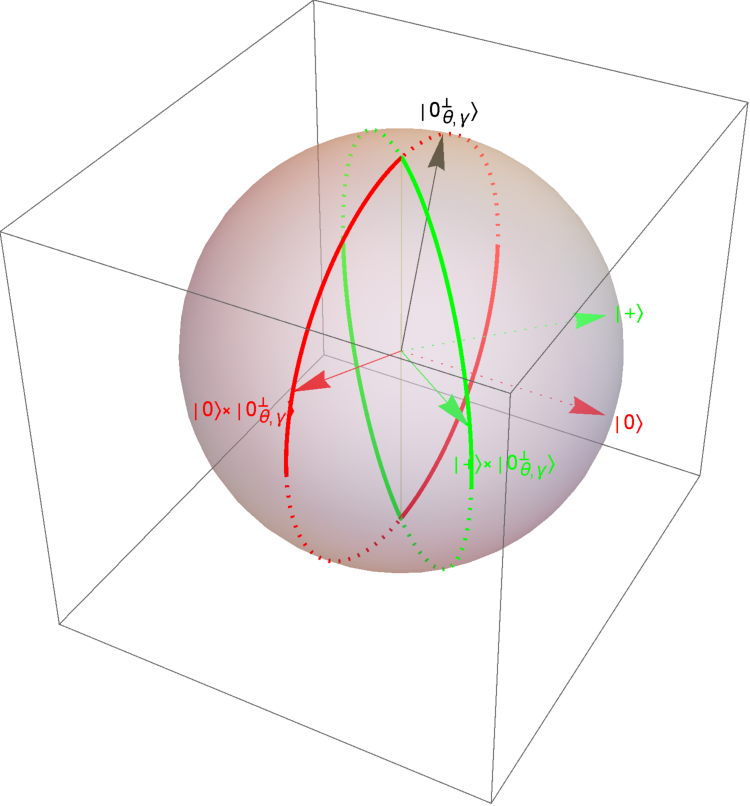
\includegraphics[scale=0.4]{measure4.pdf}
\caption{\label{fig:three-dimensional-4-value}This figure illustrates case
1 and 2 in $\mathbb{R}^{3}$ in example~\ref{ex:three-dimensional-4-value}.
The red and green dotted vector are $\ket{0}$ and $\ket{\ps}$ respectively.
All possible vectors of $\ket{0_{\theta,\gamma}^{\perp}}$ and $\ket{\ps_{\theta,\gamma}^{\perp}}$
are drawn in the red and green circles, respectively. Within the circles,
a vector~$\ket{\psi}$ in dotted part means $\bar{\mu}(\proj{\psi})=\likely$;
otherwise, $\bar{\mu}(\proj{\psi})=\unlikely$. The gray vector is
a generic vector~$\ket{0_{\theta,\gamma}^{\perp}}$, and the red
and green solid vectors are normalized $\ket{0}\times\ket{0_{\theta,\gamma}^{\perp}}$
and $\ket{\ps}\times\ket{0_{\theta,\gamma}^{\perp}}$, respectively.}
\end{figure}
\end{center}

\begin{enumerate}
\item When $\ket{\psi_{0}}$ is $\ket{0}$, then either $\ket{\psi_{1}}$
or $\ket{\psi_{2}}$ must be $\ket{0_{\theta,\gamma}^{\perp}}$ for
some $\theta$ and $\gamma$. Because of 
\[
\ket{0}\times\ket{0_{\theta,\gamma}^{\perp}}=\begin{pmatrix}1\\
0\\
0
\end{pmatrix}\times\begin{pmatrix}0\\
\rme^{\rmi\gamma}\sin\theta\\
\cos\theta
\end{pmatrix}=\begin{pmatrix}0\\
-\cos\theta\\
\rme^{-\rmi\gamma}\sin\theta
\end{pmatrix}=\rme^{-\rmi\gamma}\begin{pmatrix}0\\
\rme^{\rmi\left(\pi+\gamma\right)}\sin\left(\frac{\pi}{2}-\theta\right)\\
\cos\left(\frac{\pi}{2}-\theta\right)
\end{pmatrix}=\rme^{-\rmi\gamma}\ket{0_{\frac{\pi}{2}-\theta,\pi+\gamma}^{\perp}}
\]
the pair $\ket{\psi_{1}}=\ket{0_{\theta,\gamma}^{\perp}}$ and $\ket{\psi_{2}}=\ket{0_{\frac{\pi}{2}-\theta,\pi+\gamma}^{\perp}}$
for ($0<\theta<\frac{\pi}{2}$ and $0\le\gamma<\pi$) or $\theta=0$
enumerate all possible orthonormal bases. Equation~(\ref{eq:non-additive-vectors})
can then be verified as follow. 
\begin{equation}
\begin{aligned}\bar{\mu}\left(\mathbb{1}\tensor*[_{\mathscr{O}}]{-}{}\proj{0}\right)=\necess & \subseteq\likely\tensor*[_{\mathscr{I}}]{+}{}\unlikely=\bar{\mu}\left(\proj{0_{\theta,\gamma}^{\perp}}\right)\tensor*[_{\mathscr{I}}]{+}{}\bar{\mu}\left(\proj{0_{\frac{\pi}{2}-\theta,\pi+\gamma}^{\perp}}\right)\\
\bar{\mu}\left(\mathbb{1}\tensor*[_{\mathscr{O}}]{-}{}\proj{0_{\theta,\gamma}^{\perp}}\right)=\unlikely & =\unlikely\tensor*[_{\mathscr{I}}]{+}{}\imposs=\bar{\mu}\left(\proj{0_{\frac{\pi}{2}-\theta,\pi+\gamma}^{\perp}}\right)\tensor*[_{\mathscr{I}}]{+}{}\bar{\mu}\left(\proj{0}\right)\\
\bar{\mu}\left(\mathbb{1}\tensor*[_{\mathscr{O}}]{-}{}\proj{0_{\frac{\pi}{2}-\theta,\pi+\gamma}^{\perp}}\right)=\likely & =\imposs\tensor*[_{\mathscr{I}}]{+}{}\likely=\bar{\mu}\left(\proj{0}\right)\tensor*[_{\mathscr{I}}]{+}{}\bar{\mu}\left(\proj{0_{\theta,\gamma}^{\perp}}\right)
\end{aligned}
\label{eq:case1}
\end{equation}
Similarly, when $\ket{\psi_{0}}$ is $\ket{\ps}$, equation~(\ref{eq:non-additive-vectors})
holds. 
\item When $\ket{0}\notin\mathcal{B}$ and $\ket{\psi_{0}}=\ket{0_{\theta,\gamma}^{\perp}}$
for $0\le\theta<\frac{\pi}{2}$ and $0\le\gamma<\pi$, we want to
prove $\bar{\mu}\left(\proj{\psi_{1}}\right)=\bar{\mu}\left(\proj{\psi_{2}}\right)=\unlikely$.
Then, we have 
\begin{equation}
\begin{aligned}\bar{\mu}\left(\mathbb{1}\tensor*[_{\mathscr{O}}]{-}{}\proj{0_{\theta,\gamma}^{\perp}}\right)=\unlikely & \subseteq\unlikely\tensor*[_{\mathscr{I}}]{+}{}\unlikely=\bar{\mu}\left(\proj{\psi_{1}}\right)\tensor*[_{\mathscr{I}}]{+}{}\bar{\mu}\left(\proj{\psi_{2}}\right)\\
\bar{\mu}\left(\mathbb{1}\tensor*[_{\mathscr{O}}]{-}{}\proj{\psi_{1}}\right)=\likely & \subseteq\unlikely\tensor*[_{\mathscr{I}}]{+}{}\likely=\bar{\mu}\left(\proj{\psi_{2}}\right)\tensor*[_{\mathscr{I}}]{+}{}\bar{\mu}\left(\proj{0_{\theta,\gamma}^{\perp}}\right)
\end{aligned}
\label{eq:case2}
\end{equation}
In order to verify $\bar{\mu}\left(\proj{\psi_{1}}\right)=\bar{\mu}\left(\proj{\psi_{2}}\right)=\unlikely$,
it is sufficient to prove that if $\ket{\ps_{\theta',\gamma'}^{\perp}}\in\mathcal{B}$,
then ($0<\theta'<\frac{\pi}{2}$ and $\pi\le\gamma'<2\pi$) or $\theta'=\frac{\pi}{2}$.
Recall $\ip{\ps}{\ps_{\theta',\gamma'}^{\perp}}=0$. Hence, if $\ket{\ps_{\theta',\gamma'}^{\perp}}\in\mathcal{B}$,
we have $\ket{\ps_{\theta',\gamma'}^{\perp}}$ parallel to $\ket{\ps}\times\ket{0_{\theta,\gamma}^{\perp}}$.
\begin{equation}
\ket{\ps}\times\ket{0_{\theta,\gamma}^{\perp}}=\begin{pmatrix}1\\
1\\
0
\end{pmatrix}\times\begin{pmatrix}0\\
\rme^{\rmi\gamma}\sin\theta\\
\cos\theta
\end{pmatrix}=\begin{pmatrix}\cos\theta\\
-\cos\theta\\
\rme^{-\rmi\gamma}\sin\theta
\end{pmatrix}=\rme^{-\rmi\gamma}\begin{pmatrix}-\rme^{\rmi\left(\pi+\gamma\right)}\sin\left(\frac{\pi}{2}-\theta\right)\\
\rme^{\rmi\left(\pi+\gamma\right)}\sin\left(\frac{\pi}{2}-\theta\right)\\
\cos\left(\frac{\pi}{2}-\theta\right)
\end{pmatrix}=\sqrt{2}\rme^{-\rmi\gamma}\ket{\ps_{\frac{\pi}{2}-\theta,\pi+\gamma}^{\perp}}\label{eq:case2-cross}
\end{equation}
Because of $0\le\theta<\frac{\pi}{2}$ and $0\le\gamma<\pi$, we have
($0<\theta'=\frac{\pi}{2}-\theta<\frac{\pi}{2}$ and $\pi\le\gamma'=\pi+\gamma<2\pi$)
or $\theta'=\frac{\pi}{2}-\theta=\frac{\pi}{2}$. Similarly, when
$\ket{\psi_{0}}$ is $\ket{\ps_{\theta,\gamma}^{\perp}}$ and $\ket{\ps}\notin\mathcal{B}$,
equation~(\ref{eq:non-additive-vectors}) holds. 
\item Finally, when $\ket{0}\notin\mathcal{B}$, $\ket{\ps}\notin\mathcal{B}$,
$\ket{0_{\theta,\gamma}^{\perp}}\notin\mathcal{B}$, and $\ket{\ps_{\theta,\gamma}^{\perp}}\notin\mathcal{B}$
for $0\le\theta<\frac{\pi}{2}$ and $0\le\gamma<\pi$, i.e., the ``otherwise''
case. Then, equation~(\ref{eq:non-additive-vectors}) can easily
be verified. 
\begin{equation}
\bar{\mu}\left(\mathbb{1}\tensor*[_{\mathscr{O}}]{-}{}\proj{\psi_{0}}\right)=\likely\subseteq\unlikely\tensor*[_{\mathscr{I}}]{+}{}\unlikely=\bar{\mu}\left(\proj{\psi_{1}}\right)\tensor*[_{\mathscr{I}}]{+}{}\bar{\mu}\left(\proj{\psi_{2}}\right)\label{eq:case3}
\end{equation}
\end{enumerate}
\end{example}

The following example verifies example~\ref{ex:three-dimensional-4-value}
cannot hold with more precise intervals.

\begin{example}[Three-dimensional quantum 4-value interval-valued
probability measure (Continue)]\label{ex:three-dimensional-4-value-1}
Consider $\mathscr{I}=\left\{ \imposs,\left[l_{1},r_{1}\right],\left[1\tensor*[_{\mathbb{R}}]{-}{}r_{1},1\tensor*[_{\mathbb{R}}]{-}{}l_{1}\right],\necess\right\} $,
where $\left[l_{1},r_{1}\right]$ and $\left[1\tensor*[_{\mathbb{R}}]{-}{}r_{1},1\tensor*[_{\mathbb{R}}]{-}{}l_{1}\right]$
will be used to replace every $\unlikely$ and $\likely$ in example~\ref{ex:three-dimensional-4-value},
respectively. The bound of $l_{1}$ and $r_{1}$ can then be estimated
by the equations corresponding to equation~(\ref{eq:case1}), (\ref{eq:case2}),
and (\ref{eq:case3}).

When we replace $\unlikely$ and $\likely$ by $\left[l_{1},r_{1}\right]$
and $\left[1\tensor*[_{\mathbb{R}}]{-}{}r_{1},1\tensor*[_{\mathbb{R}}]{-}{}l_{1}\right]$,
equation~(\ref{eq:case1}) will become

\begin{equation}
\begin{aligned}\necess & \subseteq\left[1\tensor*[_{\mathbb{R}}]{-}{}r_{1},1\tensor*[_{\mathbb{R}}]{-}{}l_{1}\right]\tensor*[_{\mathscr{I}}]{+}{}\left[l_{1},r_{1}\right]\\
\left[l_{1},r_{1}\right] & \subseteq\left[l_{1},r_{1}\right]\tensor*[_{\mathscr{I}}]{+}{}\imposs\\
\left[1\tensor*[_{\mathbb{R}}]{-}{}r_{1},1\tensor*[_{\mathbb{R}}]{-}{}l_{1}\right] & \subseteq\imposs\tensor*[_{\mathscr{I}}]{+}{}\left[1\tensor*[_{\mathbb{R}}]{-}{}r_{1},1\tensor*[_{\mathbb{R}}]{-}{}l_{1}\right]
\end{aligned}
\label{eq:case1-1}
\end{equation}
which are all tautologies. Equation~(\ref{eq:case2}) will become
\begin{equation}
\begin{aligned}\left[l_{1},r_{1}\right] & \subseteq\left[l_{1},r_{1}\right]\tensor*[_{\mathscr{I}}]{+}{}\left[l_{1},r_{1}\right]\\
\left[1\tensor*[_{\mathbb{R}}]{-}{}r_{1},1\tensor*[_{\mathbb{R}}]{-}{}l_{1}\right] & \subseteq\left[l_{1},r_{1}\right]\tensor*[_{\mathscr{I}}]{+}{}\left[1\tensor*[_{\mathbb{R}}]{-}{}r_{1},1\tensor*[_{\mathbb{R}}]{-}{}l_{1}\right]
\end{aligned}
\label{eq:case2-1}
\end{equation}
which implies $l_{1}=0$. Finally, equation~(\ref{eq:case3}) will
become
\begin{equation}
\left[1\tensor*[_{\mathbb{R}}]{-}{}r_{1},1\tensor*[_{\mathbb{R}}]{-}{}l_{1}\right]\subseteq\left[l_{1},r_{1}\right]\tensor*[_{\mathscr{I}}]{+}{}\left[l_{1},r_{1}\right]\label{eq:case3-1}
\end{equation}
which implies $\frac{1}{2}\le r_{1}\le1$. Therefore, $l_{1}=0$ and
$r_{1}=\frac{1}{2}$ provides the most precise intervals which make
example~\ref{ex:three-dimensional-4-value} work, and in this case,
the intervals are $\left\{ \imposs,\unlikely,\likely,\necess\right\}
$.
\end{example}

Although it is easier to deduce an interval-valued probability measure
has an empty core by considering the state mapped to $\imposs$ as
in example~\ref{ex:three-dimensional-three-value} and \ref{ex:three-dimensional-4-value},
it is not the only way to prove an interval-valued probability measure
has an empty core. The following family of interval-valued probability
measures satisfy that $\bar{\mu}\left(P\right)=\imposs$ if and only
if $P=\mathbb{0}$, but we can still prove them have empty cores.

Although it is easier to deduce an interval-valued probability measure
has an empty core by considering the state mapped to $\imposs$ as
in example~\ref{ex:three-dimensional-three-value} and \ref{ex:three-dimensional-4-value},
it is not the only way to prove an interval-valued probability measure
has an empty core. The following family of interval-valued probability
measures satisfy that $\bar{\mu}\left(P\right)=\imposs$ if and only
if $P=\mathbb{0}$, but we can still prove them have empty cores.

%%%%%
\subsection{Proposed Activity III: Quantum Information Theorems} 

Given quantum state as interactive system
and interval-valued probability
and perhaps additionally discrete states in finite fields (try with or without)
investigate gleason (born), bell, KS, and revisit Mermin-Meyer and
other debates and paradoxes

%%%%%
\subsection{Proposed Activity IV: Computational Aspects}

If power of observer is limited with respect to power of quantum state
then quantum state can always ``fool'' you and get away with things;
you don't have the resources to catch it in an inconsistent state; if
state is interactive and always ``uncommitted'' until you make your
move you can never catch it in a lie

explain secret key exchange; if attacker has limited power cannot
crack it; complexity crucial.

may find surprises like we found with UNIQUE-SAT; not sure where that belongs 

clear goals: KS with interval probability or with quantum states as
processes

talk about finite fields; previous work; unique-sat surprise; etc

... and quantum measurement expressed using game semantics
 
This is really about unifying classical and quantum theories of
measurement. One of the most well-developed and formalized theories of
classical measurement is the one for programming language
observational contextual equivalence.


This worldview can be maintained as long as the impact of the
measurements is really negligible on the execution time of the
functions of interest.

measurement affects runtime and hence affects other measurements;
could even conceive of programs whose input-output behavior is
affected by measurement

This intended level of abstraction is reflected in the first
line of the function declaration in Haskell. This \emph{interface} (or \emph{type}
or \emph{signature} or \emph{contract}) line:
\begin{quote}
\begin{verbatim}
square :: Int -> Int
\end{verbatim}
\end{quote}
summarizes the publicly stated, computationally relevant, aspects of the
function. In this case, it is announced that the function is a computer
realization of a pure mathematical map from one \verb|Int| to another. The
fact that executing the computer realization of the map on a particular input
might consume 10\% of the battery power on your laptop is something
that---although potentially critical knowledge in some circumstances---is not
even expressible in the notation above. 

%%-------------------------------------
\subsection*{Partial Functions (Time)}

Computations take time. At some level of abstraction, we can ignore the time
taken by a computation. For example, we can pretend that a calculation that
takes one or two microseconds is similar to the ``instantaneous'' lookup in a
mathematical mapping. But we can hardly keep pretending this as the time used
by the calculation tends towards infinity.

Consider the following Java method:
\begin{quote}
\begin{verbatim}
int collatz (int n) {
  if (n == 1) return 0; 
  else if (n % 2 == 0) return 1 + collatz (n / 2);
  else return 1 + collatz (3 * n + 1);
}
\end{verbatim}
\end{quote}
As evident from the use of \verb|collatz| in the body of the method, this
method is \emph{recursive}. It takes an input number \verb|n| and:
\begin{itemize}
\item if the input number is equal to one, the method immediately stops with
the value zero, which represents in this case the total number of recursive
calls performed before stopping;
\item if the input number is even, the method divides it by two and
recursively invokes itself, adding one to the total number of recursive
calls;
\item if the input number is odd, the method multiplies it by three, adds
one, and then recursively invokes itself, after again adding one to the total
number of recursive calls.
\end{itemize}
It is a famous mathematical conjecture, \emph{the Collatz conjecture}, that
this calculation always terminates for all positive integers. One can quickly
check a few cases:
\begin{itemize}
\item invoking \verb|collatz(3)| iterates through 10, 5, 16, 8, 4, 2, 1, and
  then stops returning the result 7.
\item invoking \verb|collatz(17)| iterates through 52, 26, 13, 40, 20, 10, 5,
16, 8, 4, 2, 1, and then stops returning the result 12.
\end{itemize}

There is however no known proof that this method always stops. Thus, even
though the method has the same interface as the method \verb|square| above,
one may not be able to interpret the two interfaces in the same way. To
account for the possibility that the calculation never stops, the interface:
\begin{quote}
\begin{verbatim}
int collatz (int n)
\end{verbatim}
\end{quote}
should in general be read as saying:
\begin{quote}
Given a particular \verb|int| the method \emph{may or may not} return another
\verb|int| in a finite amount of time.
\end{quote}

Another way to look at the situation is that we have introduced ``time'' as
an implicit parameter of computations. Some computations as the method
\verb|square| update---as a side effect---this time parameter by consuming a
few ticks. By general agreement, this consumption is deemed negligible and
not ``observable'' and does not generally constitute a computational
effect. But when the consumption of time is unbounded, it arguably becomes an
observable computational effect.

%%-------------------------------------
\subsection*{Assignments (Memory)}

Computations require memory. Again, at some level of abstraction we can
pretend that memory does not exist. But what happens if a computation
starts changing external memory locations? 

Consider the following variant of the method \verb.square.:
\begin{quote}
\begin{verbatim}
int square (int n) {
  count++;
  return n * n;
}
\end{verbatim}
\end{quote}
As before, the method takes an integer \verb.n. from the domain of Java
integers \verb.int. and returns another integer whose value is the square of
the input. But, as a side effect the method reads and updates an external
reference \verb.count., which can be used to find out how many times the
method was called. Thus if during the execution of a particular program the
method \verb.square. is called ten times, then the value of \verb.count. will
be ten.

Thus the interface:
\begin{quote}
\begin{verbatim}
int square (int n)
\end{verbatim}
\end{quote}
should now be read as saying:
\begin{quote}
Given a particular \verb|int| the method \emph{may possibly} read and update
external memory references and then it \emph{may or may not} return another
\verb|int| in a finite amount of time.
\end{quote}

Another way to look at the situation is that we have introduced ``memory'' as
an implicit parameter of computations. Some computations as the original
method \verb|square| might---as a side effect---allocate, update, and read
several memory locations (registers, cache entries, stack frames, etc.). By
general agreement, these actions on memory are not considered observable and
do not generally constitute a computational effect. But when a computation
updates an external memory location that other program fragments can inspect,
the update of the memory location becomes an observable computational effect.

%%-------------------------------------
\subsection*{Runtime Exceptions (Context)}

Computations occur in a context. When a computation occurs in the context of
a larger computation, it is typically expected to return its result to that
outer computation. But what if a computation cannot return a sensible value
to its context and decides instead to abort it?

Consider again the method \verb|square| whose interface is:
\begin{quote}
\begin{verbatim} 
int square (int n)
\end{verbatim}
\end{quote}
We initially argued that it is possible to interpret this interface to say
that given a particular \verb|int| the method's execution promises to return
another \verb|int|. This is clearly an idealized view: in real life, any of
an unlimited number of failures may occur in the hardware or underlying
software components including the operating system or the Java virtual
machine. The Java language collectively refers to these conditions as
\verb|Error|s or \verb|RuntimeException|s.

So to be more accurate, and putting together our observations so far, one
should interpret the interface:
\begin{quote}
\begin{verbatim} 
int square (int n)
\end{verbatim}
\end{quote}
as saying:
\begin{quote}
Given a particular \verb|int| the method \emph{may possibly} read and
update external references, and then it \emph{may or may not} return another
\verb|int| in a finite time or it \emph{may fail to return to its context}
due to any of a number of errors and runtime exceptions.
\end{quote}

Another way to look at the situation is that we have introduced the
``context'' as an implicit parameter of computations. It is expected that
every inner computation would resume its context with its result. But when an
inner computation encounters a fatal error condition, it can ignore the
context parameter, which causes the error condition to immediately terminate
the entire computation. This escape clearly constitutes an observable
computational effect.

%%-------------------------------------
\subsection*{Other Computational Effects}

The unifying theme in all the above effects is that computations do not
happen in isolation in some abstract mathematical world: rather computations
are realized in some physical computing platform. The physical interactions
of a computation with the computing platform and with other computations may
be ignored in some idealized situation corresponding to simple computations,
but they become crucial if one is interested in modeling the actual behavior
of a sophisticated realistic computation. If these interactions happen
``behind the scene'' they are considered side effects of the computation.

Without further constraints on computations and their contexts, it is
impossible to enumerate all the possible side effects that a computation may
have. The reader may find it instructive to consider the following list of
effects that could be performed by a method with the interface:
\begin{quote}
\begin{verbatim} 
int square (int n)
\end{verbatim}
\end{quote}
Given a particular \verb|int|, the method's behavior may include various
combinations of the following actions:
\begin{itemize}
\item Reading and updating external memory locations, environment parameters,
local or remote file systems or databases, etc.
\item Communicating with a user or another local or remote process.
\item Suspending itself for a certain period of time or until a certain
outside condition happens.
\item Resuming other suspended computations.
\item Loading, compiling, and executing some other computation.
\item Using reflection to examine and perhaps modify its own machine
representation.
\item Producing multiple answers by arranging for one \verb|int| to be
returned now and subsequent answers to be returned when the method is called
again (with the same parameters). 
\item Checkpointing its entire state to a log, which can be examined and
resumed later.
\item Failing due to any of a number of errors and runtime exceptions.
\item Consuming half of the battery life of a laptop and generating enough
heat to keep you warm on a cold winter night.
\end{itemize}
And yes by the way, the method may actually return another \verb|int| in a
finite amount of time.

It is clear that the method's interface is nowhere close to giving us a
reasonable approximation of the possible behaviors of the method: it sweeps
too many things under the rug. Pragmatically, if a programmer invokes a
method with the interface:
\begin{quote}
\begin{verbatim} 
int square (int n)
\end{verbatim}
\end{quote}
the implicit computational effects of the method might come as a
surprise. 

The situation is not unique to Java. Almost every other programming
language allows similar computational effects to occur
implicitly. Even hardware circuits and assembly language instructions
often perform implicit effects. For example, an assembly instruction
might change the contents of the flag register as a side effect. In
fact natural languages also include various ``non-compositional
phenomena,'' which are essentially computational effects. For this
reason, programmers are universally taught to avoid side effects if
possible and to be careful when analyzing code that might contain side
effects. But when side effects are unavoidable, the solution is to
\emph{expose them} as the rest of the article explains.

Common wisdom is that classical physics has no randomness. Only
ignorance of the fine details or lack of control over them causes
\emph{statistical randomness}. In principle, but not in practice,
randomness is absent from classical physics.

In sharp contrast, quantum randomness is unavoidable even in principle. 

But but but ... Nature is one. The distinction between ``classical''
and ``quantum'' can only be in our minds, or more precisely in our
mathematical models of the universe. We have two mathematical models,
one which is, in principle deterministic, and one which is
probabilistic. Nature must really be one or the other.

Consider this unsettling quote from QBism:

\begin{quote} 
Instead, the wavefunction obeys two fundamentally different laws:
\begin{enumerate}
\item As long as the electron is left to its own devices unobserved
  its wavefunction unfolds smoothly, continuously, and predictably. It
  obeys fixed mathematical laws, just like a bullet in flight and a
  wave on a lake.
\item When the electron reveals its whereabouts by leaving a dot on a
  screen, the wavefunction ``collapses'' suddenly into a new much more
  compact form concentrated on the point of impact.
\end{enumerate}

\end{quote}

Can we develop a mathematical model that unifies both the classical
deterministic perspective and the quantum probabilistic perspective?
Quantum information and quantum computation opens the door to using
computational insights. The main one is that, in a computation,
everything produced during a computation and everything observed about
a computation is finite. The computational perspective imposes a
principle we might call the principle of ``finitely communicable
evidence.''

So imprecision in classical physics becomes, not some second-class
principle that is considered to stem from practical limitations but
rather a foundational principle. If everything is ``fuzzy'' so to
speak and if our mathematical models embrace this fuzziness then a
different worldview emerges. That worldview agrees with classical
physics but embraces imprecision within the mathematical model not as
an external non-mathematical nuisance. This shift in perspective
enables a smooth transition to the world of quantum physics since our
mathematical model has already embraced probabilistic effects.

Three insights:

\begin{itemize}
\item Interactive systems: response of quantum system determined
  \emph{after} the observer initiates the experiment used to observe
  the system
\item Bayesian probability, personal
\item Finite precision
\end{itemize}

Goal: build computational model of QM that encompasses classical
(reversible), computation and observation with finite resources, and
hopefully revolutionize ``quantum thinking''

%%%%%%%%%%%%%%%%%%%%%%%%%%%%%%%%%%%%%%%%%%%%%%%%%%%%%%%%%%%%%%%%%%%%%%%%%%%%%%
\section{Broader Impact and Education} 

%%%%%%%%%%%%%%%%%%%%%%%%%%%%%%%%%%%%%%%%%%%%%%%%%%%%%%%%%%%%%%%%%%%%%%%%%%%%%%
\section{PI Team and Prior NSF Support} 

Over the past several years, the PI, together with other IU faculty
members and students, has formed a group whose main interest is the
study of paradigms of computing that either arise in nature or are
inspired by natural phenomena. The PI is especially interested in how
the laws of physics can inspire and guide our abstract computational
models, as well as exposing new insights into the computational
framework behind the natural world and the computability of physical
theory. Our group has been active in several areas related to the
theory behind quantum computation. Particular areas include:
mathematical foundations of quantum computation and
complexity~\cite{AGVS2007,VAS2006},
adiabatic quantum computing, quantum logic, classical and quantum
reversible programming languages~\cite{Sabry:2003:MQC:871895.871900},
analog computation and its limits, and optical computing. During the
last year, our discussions have revolved around formulating variants
of quantum mechanics that are computable and that are as close to
possible to classical computing. Several preliminary results have
emerged from our collaboration~\cite{usat,finiteQC,geometry2013,DQT2014}, and the group
is very excited about the potential implications of those
results. This proposal brings forth a particular aspect of this
programme related to its applications to problem areas that have
traditionally been outside the conceptual framework of programming
language research.

In the past five years, Prof. Sabry received one NSF grant (award
number 1217454) titled \emph{Information Effects} for the amount of
\$275,319.00 with start and end dates of 1 September 2012 -- 31 August
2016.

% (c) a summary of the results of the completed work, including
% accomplishments, supported by the award. The results must be
% separately described under two distinct headings, Intellectual Merit
% and Broader Impacts;

% (d) a listing of the publications resulting from the NSF award (a
% complete bibliographic citation for each publication must be provided
% either in this section or in the References Cited section of the
% proposal); if none, state "No publications were produced under this
% award."

% (e) evidence of research products and their availability, including,
% but not limited to: data, publications, samples, physical collections,
% software, and models, as described in any Data Management Plan; and

\paragraph*{Intellectual Merit.}                                                 
                                                                     
\paragraph*{Broader Impacts.}                                                    
                                                                                
%%%%%%%%%%%%%%%%%%%%%%%%%%%%%%%%%%%%%%%%%%%%%%%%%%%%%%%%%%%%%%%%%%%%%%%%%%%%%%
\newpage
\printbibliography
\end{document}

%%%%%%%%%%%%%%%%%%%%%%%%%%%%%%%%%%%%%%%%%%%%%%%%%%%%%%%%%%%%%%%%%%%%%%%%%%%%%%



